\thispagestyle{empty}

\noindent
\begin{tabular}{@{}p{11cm}r@{}}
\textbf{ಡಾ. ಎ.ವಿ. ಪ್ರಸನ್ನ, {\fontsize{7pt}{9pt}\selectfont ಎಂ.ಎ., ಡಿ.ಲಿಟ್​, ಎಲ್​.ಎಲ್​.ಬಿ.}\relax}\newline ನಿವೃತ್ತ ಹಿರಿಯ ಕೆ.ಎ.ಎಸ್​. ಅಧಿಕಾರಿಗಳು,\newline ಗೌರವ ಪ್ರಾಧ್ಯಾಪಕರು, ಕುಮಾರವ್ಯಾಸ ಪೀಠ, ತುಮಕೂರು ವಿಶ್ವವಿದ್ಯಾನಿಲಯ\newline ಸುಪ್ರಸಿದ್ದ ಗಮಕಿಗಳು, ವ್ಯಾಖ್ಯಾನಕಾರರು & \raisebox{-2cm}{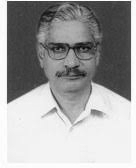
\includegraphics[scale=.75]{"images/prasanna.jpeg"}}
\end{tabular}

\noindent
\rule{\textwidth}{1pt}

\vskip .2cm

\centerline{\textbf{ಆಶಯದ ನುಡಿಗಳು}}

\vskip .2cm

ಒಂದು ಪ್ರದೇಶದ ಇತಿಹಾಸ, ರಾಜಕಿಯ, ಜನಜೀವನ ಸಾಹಿತ್ಯ, ಸಂಸ್ಕೃತಿ ಮುಂತಾದವುಗಳ ಅಧ್ಯಯನಕ್ಕೆ ಶಾಸನಗಳೇ ಮೂಲಾಧಾರ ಸ್ವರೂಪದಲ್ಲಿರುತ್ತವೆ. ಸಾವಿರಾರು ವರ್ಷಗಳ ಇತಿಹಾಸವಿರುವ ಭಾರತದಂತಹ ದೇಶಗಳಿಗೆ ಶಾಸನಗಳು ಮತ್ತು ಪ್ರಾಚೀನ ಸಾಹಿತ್ಯಗಳೇ ಸಾಂಸ್ಕೃತಿಕ ಆಸ್ತಿಗಳು. ಶಾಸನಗಳು ಜನತೆಯ ಜೀವನದ ಲಿಖಿತ ಪ್ರತಿಬಿಂಬ\-ಗಳಾಗಿವೆ. ಈ ಮಾತುಗಳಿಗೆ ಶ‍್ರೀ ಸಂತೇಬಾಚಹಳ್ಳಿ ನಂಜುಂಡಸ್ವಾಮಿಯವರ “ಮಂಡ್ಯ ಜಿಲ್ಲೆಯ ಶಾಸನಗಳು ಒಂದು ಅಧ್ಯಯನ” ಎಂಬ ಮಹಾಪ್ರಬಂಧವು ಒಂದು ನಿದರ್ಶನವಾಗಿದೆ. ಈ ಮಹಾ ಪ್ರಬಂಧವನ್ನು ಓದಿದಾಗ ಇದರ ಬೃಹತ್ತು, ಮಹತ್ತುಗಳು ಮತ್ತು ವಿಷಯ ವೈವಿಧ್ಯಗಳು ಆಶ್ಚರ್ಯ\-ವನ್ನುಂಟು ಮಾಡುತ್ತವೆ. ಶ‍್ರೀ ನಂಜುಂಡಸ್ವಾಮಿಯವರು ಪಿ.ಹೆಚ್​.ಡಿ ಪದವಿ\-ಗಾಗಿ ಈ ಅಧ್ಯಯನವನ್ನು ಕೈಗೊಂಡು ಈ ಮಹಾ ಪ್ರಬಂಧವನ್ನು ರಚಿಸಿರುತ್ತಾರೆ. ಆದರೆ ಇದು ಕೇವಲ ಈ ಪದವಿಗಾಗಿ ಮಾತ್ರ ಮಾಡಿರುವ ಅಧ್ಯಯನವಲ್ಲ. ಕಳೆದ ಸುಮಾರು ಮೂವತ್ತು ವರ್ಷಗಳಷ್ಟುಕಾಲ ಸುದೀರ್ಘವಾದ ಅಧ್ಯಯನ ಮಾಡಿ, ಆ ಅನುಭವದಿಂದ ರಚಿತಗೊಂಡಿರುವ ಗ್ರಂಥವಿದು. ಸಾಮಾನ್ಯವಾಗಿ ಮಾನವಿಕ ವಿಭಾಗ ಮತ್ತು ಸಾಹಿತ್ಯ ಸಂಬಂಧೀ ಸಂಶೋಧನಾತ್ಮಕ ಬರಹಗಳು ಕೇವಲ ಗ್ರಂಥಾಲಯ\-ಗಳೊಳಗಿನ ಅಧ್ಯಯನದಿಂದ ಸಿದ್ಧವಾಗುವುದು ವಾಡಿಕೆ. ಆದರೆ ಶ‍್ರೀ ಸಂತೇಬಾಚಹಳ್ಳಿ ನಂಜುಂಡಸ್ವಾಮಿ\-ಯವರ ಈ ಸಂಶೋಧನಾ ಪ್ರಬಂಧದ ಹಿಂದೆ, ಶಾಸನಗಳು ದೊರಕಿರುವಲ್ಲಿಗೆ ಭೇಟಿ ನೀಡಿ ಅಲ್ಲಿನ ಸುತ್ತ ಮುತ್ತ\-ಲಿನ ಸಂಗತಿ\-ಗಳನ್ನು ಅಧ್ಯಯನ ಮಾಡಿ, ಸ್ಥಳೀಯ ಜನರೊಂದಿಗೆ ಸಮೂಲೋಚಿಸಿ ಮಾಹಿತಿಗಳನ್ನು ಕಲೆ ಹಾಕಿ, ಸಂಬಂಧಿಸಿದ ಭಾವಚಿತ್ರ\-ಗಳನ್ನು ತೆಗೆದು ಅವುಗಳನ್ನು ಕ್ರೋಢೀಕರಿಸಿ ವಿಷಯವಾರು ಬರಹರೂಪಕ್ಕೆ ಇಳಿಸುವ ಪರಿಶ್ರಮ ಎದ್ದು ಕಾಣುತ್ತದೆ. ಇದು ಅಪಾರ ಶ್ರಮ\-ವನ್ನು ಮತ್ತು ಶ್ರದ್ಧೆಯನ್ನು ಬೇಡುವ ಕೆಲಸ. ಸಂಶೋಧನಕಾರರು ಇದನ್ನು ಅತ್ಯಂತ ಸಮರ್ಪಕವಾಗಿ ಮಾಡಿದ್ದಾರೆಂಬುದು ಗ್ರಂಥದ ಪ್ರತಿ ಪುಟದಲ್ಲಿಯೂ ಗೋಚರವಾಗುತ್ತದೆ. ಮಂಡ್ಯ ಜಿಲ್ಲೆಯ ಸಮಗ್ರ ಪ್ರಾಚಿನ ಇತಿಹಾಸವೇ ಇಲ್ಲಿ ದಾಖಲಾಗಿದೆಯಂದರೆ ಅತಿಶಯೋಕ್ತಿಯಲ್ಲ. ಇಂತಹ ಒಂದು ಶ್ರೇಷ್ಠ ಗ್ರಂಥವನ್ನು ರಚಿಸುವ ಮೂಲಕ ಕನ್ನಡ ನಾಡಿನ ಸಮಗ್ರ ಜನತೆಗೆ ಪ್ರಾಚೀನ ಮಂಡ್ಯ ಜಿಲ್ಲೆಯ ಸಾಂಸ್ಕೃತಿಕ ವೈಭವವನ್ನು ಶ‍್ರೀ ನಂಜುಂಡಸ್ವಾಮಿಯವರು ಪರಿಚಯ ಮಾಡಿ ಕೊಟ್ಟಿದ್ದಾರೆ. ಇದು ಮಂಡ್ಯದ ಭಾಗ್ಯದಿಂದ ರಚಿತವಾದ ಕೃತಿ. ಮಂಡ್ಯ ಜಿಲ್ಲೆಯ ಕೃತಜ್ಞತೆ ಲೇಖಕರಿಗೆ ಸಲ್ಲಬೇಕು. ಮಂಡ್ಯ ಜಿಲ್ಲೆಯ ಶಾಸನಗಳ ಈ ಸಮಗ್ರ ಅಧ್ಯಯನವು ರಾಜ್ಯದ ಇತರ ಜಿಲ್ಲೆಗಳ ಬಗ್ಗೆ ಸಹ ನಡೆಯಲು ಮಾರ್ಗದರ್ಶನ ಮತ್ತು ಸ್ಪೂರ್ತಿಯನ್ನು ನೀಡುವುದರಲ್ಲಿ ಸಂಶಯವಿಲ್ಲ. ಈಗ ಈ ಮಹಾಪ್ರಬಂಧವು ಪರಿಷ್ಕೃತಗೊಂಡು “ಮಂಡ್ಯ ಜಿಲ್ಲೆಯ ಶಾಸನ ಮತ್ತು ಸಂಸ್ಕೃತಿ” ಎಂಬ ಹೆಸರಿನಿಂದ ಗ್ರಂಥರೂಪದಲ್ಲಿ ಪ್ರಕಟವಾಗುತ್ತಿದೆ. ಶಾಸನ ಸಾಹಿತ್ಯದ ಮತ್ತು ಸಂಶೋಧನ ಕ್ಷೇತ್ರದ ವಿದ್ಯಾರ್ಥಿಗಳು ಮತ್ತು ಆಸಕ್ತ ಸಾರ್ವ\-ಜನಿಕರು ಇದರ ಸಂಪೂರ್ಣ ಪ್ರಯೋಜನವನ್ನು ಪಡೆಯಲೆಂದು ಆಶಿಸುತ್ತೇನೆ. ಸನ್ಮಿತ್ರರಾದ ಶ‍್ರೀ ಸಂತೇಬಾಚಹಳ್ಳಿ ನಂಜುಂಡಸ್ವಾಮಿ ಅವರ ಅನೇಕ ಲೇಖನಗಳಿಂದ ಮತ್ತು ಮಾಹಿತಿಗಳಿಂದ ಉಪಕೃತನಾಗಿದ್ದೇನೆಂಬು\-ದನ್ನು ಸ್ಮರಿಸುತ್ತಾ ಗ್ರಂಥ ಬಿಡುಗಡೆಯ ಈ ಶುಭಾವಸರದಲ್ಲಿ ಅವರಿಗೆ ಹಾರ್ದಿಕ ಅಭಿನಂದನೆಗಳನ್ನು ಸಲ್ಲಿಸುತ್ತೇನೆ.


\bigskip

\noindent
ಬೆಂಗಳೂರು - 94\hfill \textbf{ಡಾ. ಎ.ವಿ. ಪ್ರಸನ್ನ}

\vskip -.2cm

\noindent
 ದಿನಾಂಕ: 14-12-2018

